\documentclass{ximera}
\title{Exercises: Disks and Washers}
\author{Philip T. Gressman}

\begin{document}
\begin{abstract}
Exercises for the disk and washer methods.
\end{abstract}
\maketitle

\begin{exercise}
The region $0 \leq y \leq \sqrt{x}$ with $x \leq 1$, shown below, is revolved around the $x$-axis. Use the disk method to find the volume of the solid of revolution.
\begin{center}
\begin{image}
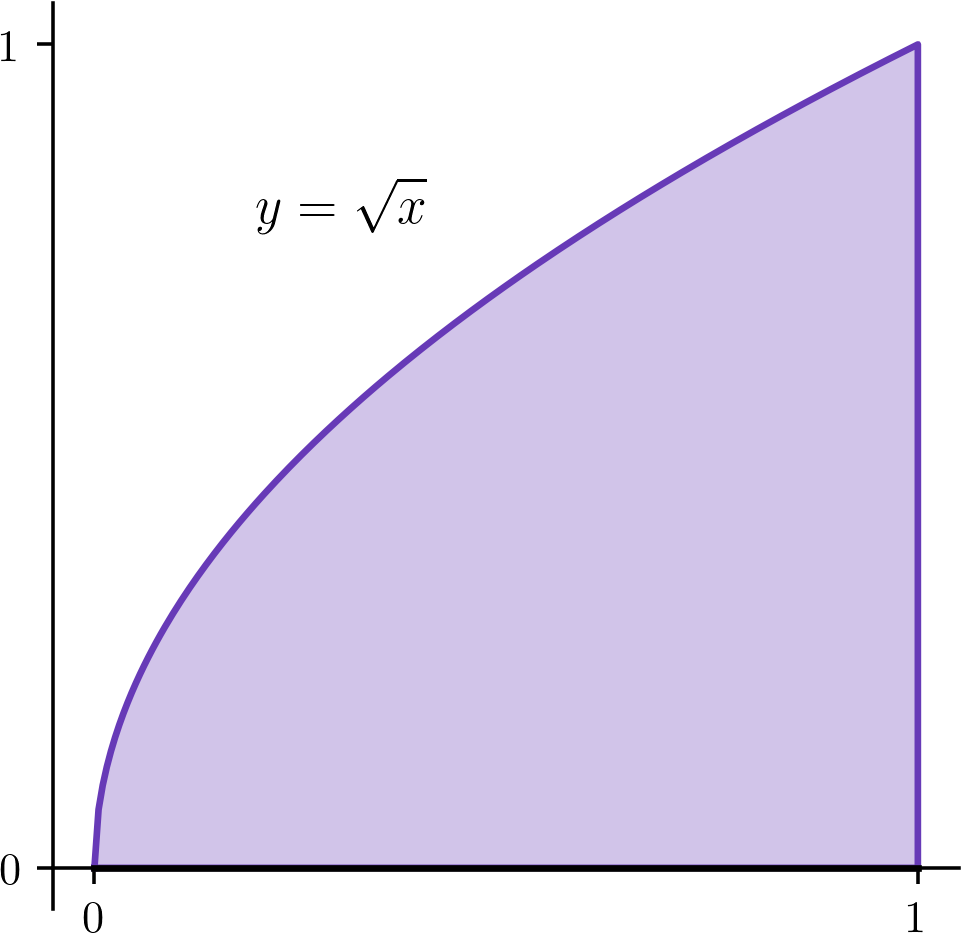
\includegraphics[width=4in]{diskwasher/disk01.png}
\end{image}
\end{center}
\begin{hint}
The radius $R(x)$ will be a difference of $y$-values because slices are indexed by the variable $x$.
Each slice will extend from $y=0$ to $y =  \sqrt{x}$, and so $R(x)$ must be the larger of these $y$-values minus the smaller of these $y$-values.
\end{hint}
\begin{prompt}
\[ R(x) = \answer{\sqrt{x}} \]
\[ V = \int_{\answer{0}}^{\answer{1}} \pi (R(x))^2 dx =  \answer{\frac{\pi}{2}} \]
\end{prompt}
\end{exercise}


\begin{exercise}
The region $0 \leq y \leq \sqrt{x}$ with $x \leq 1$, shown below, is revolved around the axis $x=1$. Use the disk method to find the volume of the solid of revolution.
\begin{center}
\begin{image}
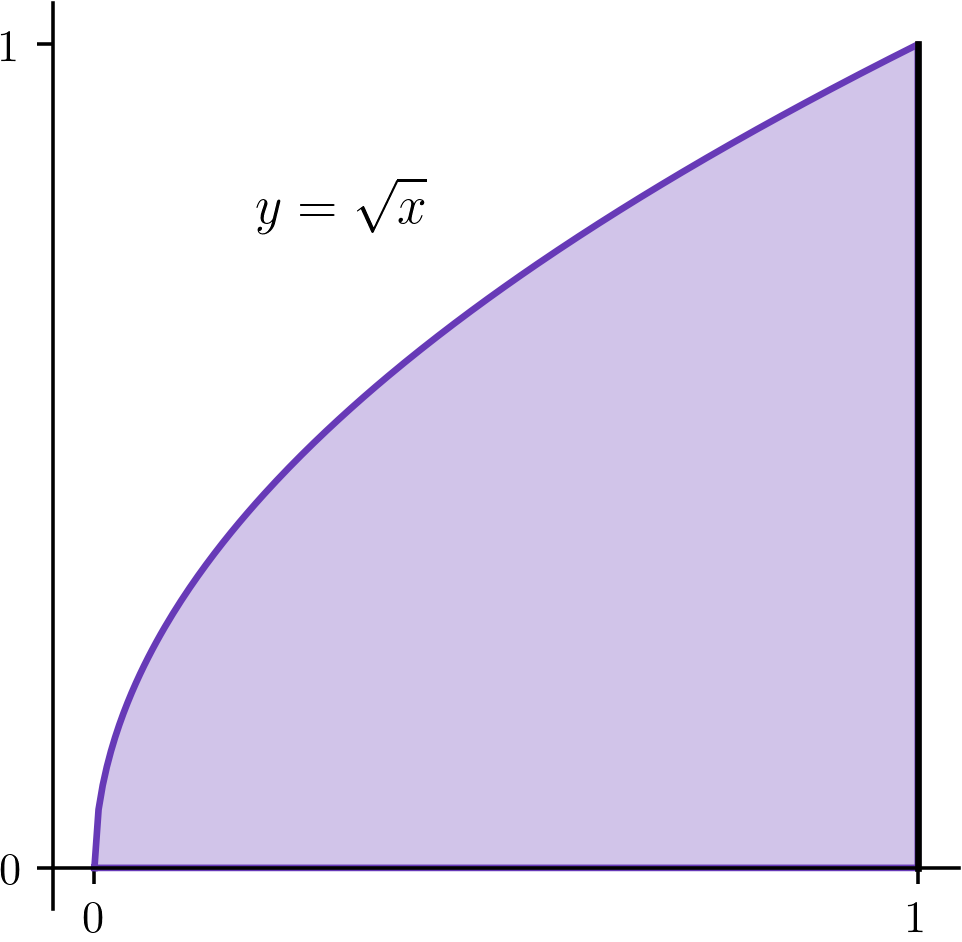
\includegraphics[width=4in]{diskwasher/disk02.png}
\end{image}
\end{center}
\begin{hint}
The radius $R(y)$ will be a difference of $x$-values because slices are indexed by the variable $y$.
Each slice will extend from $x = y^2$ to $x = 1$, and so $R(y)$ must be the larger of these $x$-values minus the smaller of these $x$-values
\end{hint}
\begin{prompt}
\[ R(y) = \answer{1 - y^2} \]
\[ V = \int_{\answer{0}}^{\answer{1}} \pi (R(y))^2 dy = \answer{\frac{8\pi}{15}} \]
\end{prompt}
\end{exercise}


\begin{exercise}
The region $0 \leq y \leq \sqrt{x}$ with $x \leq 1$, shown below, is revolved around the axis $x=0$. Use the washer method to find the volume of the solid of revolution.
\begin{center}
\begin{image}
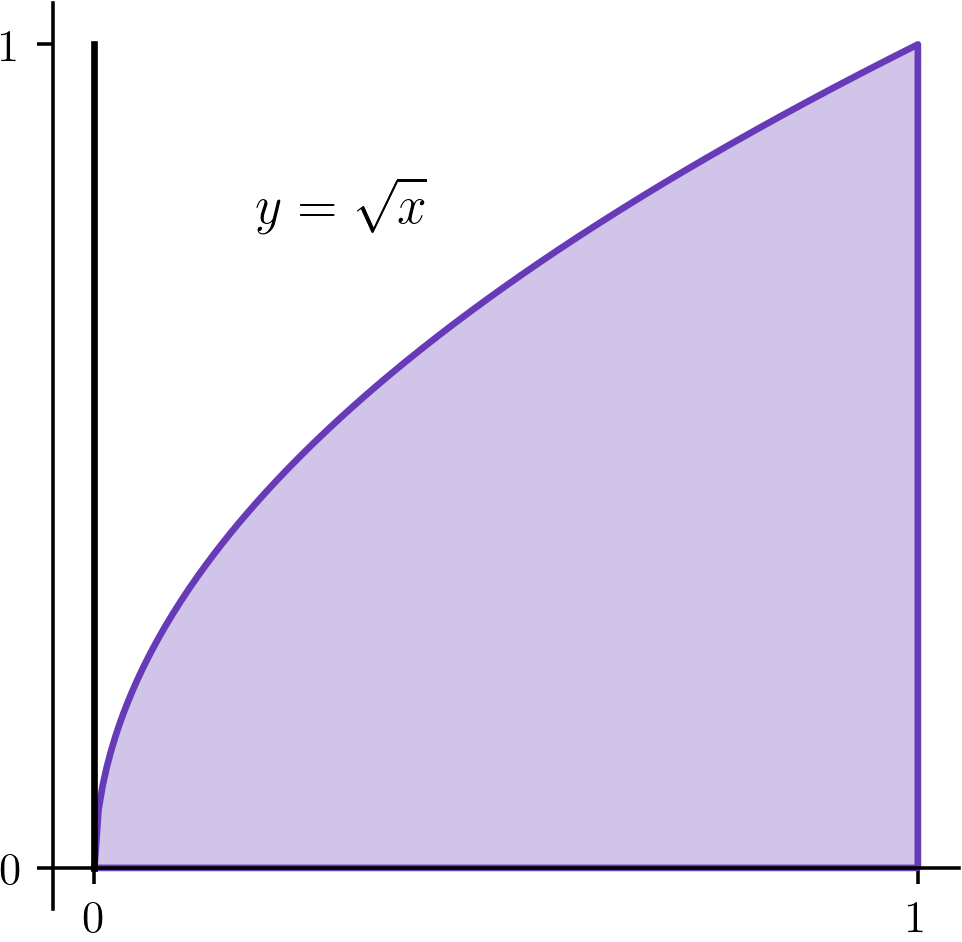
\includegraphics[width=4in]{diskwasher/disk04.png}
\end{image}
\end{center}
\begin{hint}
Each radius will be a difference of $x$-values because slices are indexed by the variable $y$.
The distance from the axis $x=0$ to the line $x=1$ is $1$, and the distance from the axis $x=0$ to $x = y^2$ is $y^2$.
\end{hint}
\begin{prompt}
\[ R_{\mathrm{outer}} (y) = \answer{1} \text{ and } r_{\mathrm{inner}}(y) = \answer{y^2} \]
\[ V = \int_{\answer{0}}^{\answer{1}} \pi  \left[ (R_{\mathrm{outer}}(y))^2 - (r_{\mathrm{inner}}(y))^2 \right] dy =  \answer{\frac{4\pi}{5}} \]
\end{prompt}

\end{exercise}

\begin{exercise}
The region $0 \leq y \leq \sqrt{x}$ with $x \leq 1$, shown below, is revolved around the axis $y=1$. Use the washer method to find the volume of the solid of revolution.
\begin{center}
\begin{image}
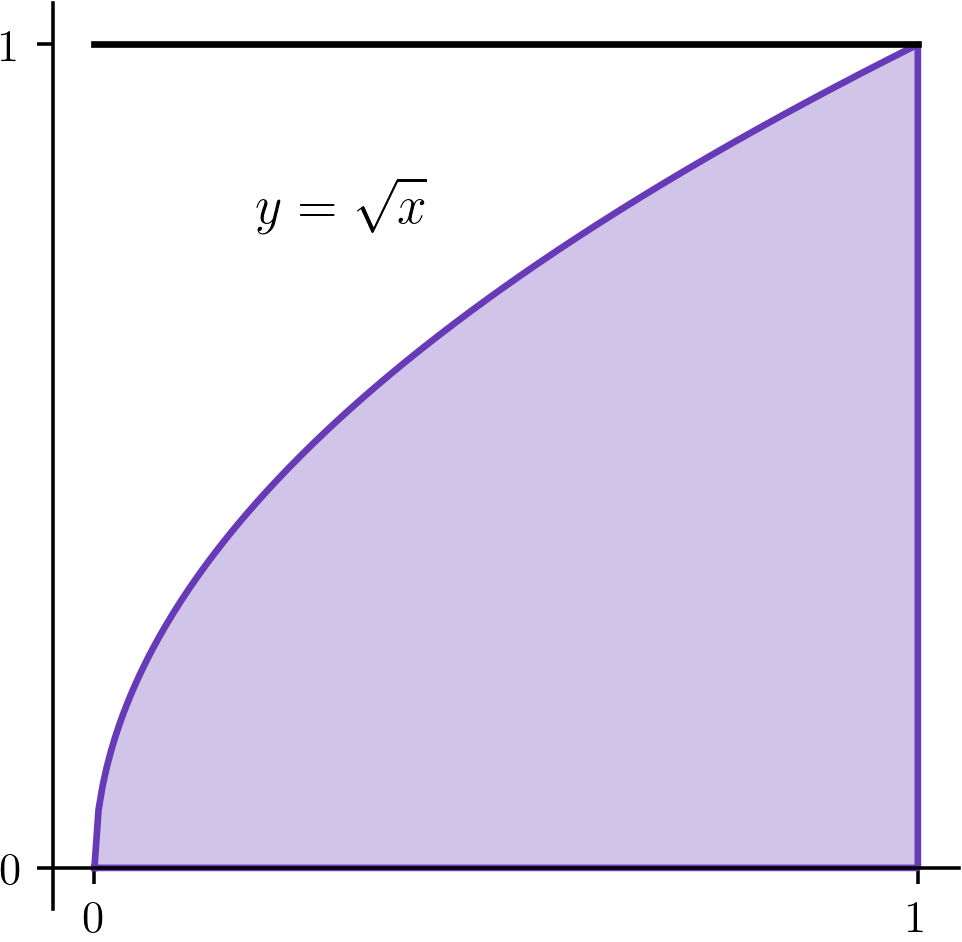
\includegraphics[width=4in]{diskwasher/disk03.png}
\end{image}
\end{center}
\begin{hint}
Each radius will be a difference of $y$-values because slices are indexed by the variable $x$.
The distance from the axis $y=1$ to the line $y=0$ is $1$, and the distance from the axis $y=1$ to $y = \sqrt{x}$ is $1 - \sqrt{x}$.
\end{hint}
\begin{prompt}
\[ R_{\mathrm{outer}} (x) = \answer{1} \text{ and } r_{\mathrm{inner}}(x) = \answer{1-\sqrt{x}} \]
\[ V = \int_{\answer{0}}^{\answer{1}} \pi  \left[ (R_{\mathrm{outer}}(x))^2 - (r_{\mathrm{inner}}(x))^2 \right] dx =  \answer{\frac{5\pi}{6}} \]
\end{prompt}
\end{exercise}






\end{document}
